% \chapter{撰写正文}

% \section{研究生学位论文的一般格式与顺序}

% 根据《东南大学研究生学位论文格式规定》\cite{seugs2015rule}第一条之要求,研究生学位论文一般应由如下部分组成:

% \begin{enumerate}
%   \item 中文封面
%   \item 中文页面
%   \item 英文封面
%   \item 论文独创性声明和使用授权声明
%   \item 中文内容提要及关键词
%   \item 英文内容提要及关键词
%   \item 目录
%   {\color{cyan} \item 符号、变量、缩略词等本论文专用术语注释表}
%   \item 正文
%   \item 致谢
%   \item 参考文献
%   {\color{cyan} \item 附录
%   \item 中英文索引
%   \item 作者简介(包括在学期间发表的论文和取得的学术成果清单)
%   \item 后记}
% \end{enumerate}
% 上述各部分得按照此顺序排列,其中{\color{cyan} 青色}标注的部分为可选部分。我们已经在第\ref{chp:initialization}章中介绍了上述列表中第1-3项关于封面中各条目的填写与生成方法。在本章中,我们将介绍如何撰写论文的正文以及其他部分。

% \section{独创性与授权声明}

% 紧接在中英文封面后的应该是论文的独创性声明和使用授权声明,具体的文本内容请参考《学位论文独创性和使用授权声明》\cite{seugs2018license}。

% 本模板已经包含了对独创性声明和授权声明的自动生成,当编译引擎执行到

% \begin{tcolorbox}
% \begin{lstlisting}[language=TeX]
% \makebigcover
% \makecover
% \end{lstlisting}
% \end{tcolorbox}

% \noindent 时会自动到目录下的seumasterthesis.cfg文件中寻找独创性与授权声明的预定义文本。

% \section{中英文摘要}

% 《东南大学研究生学位论文格式规定》\cite{seugs2015rule}的第一条第二款中对论文摘要有如下要求:

% ~

% {\color{black!45}
% \noindent 论文摘要中文约500字左右,英文约200-300词左右,二者应基本对应。它是论文内容的高度概括,应说明研究目的、研究方法、成果和结论,要突出本论文的创造性成果或新的见解,用语简洁、准确。论文摘要后还应注明本文的关键词3-5个。关键词应为公知公用的词和学术术语,不可采用自造字词和略写、符号等,词组不宜过长。

% \noindent 英文摘要采用第三人称单数语气介绍该学位论文内容,目的是便于其他文摘摘录,因此在写作英文文摘时不宜用第一人称的语气陈述。叙述的基本时态为一般现在时,确实需要强调过去的事情或者已经完成的行为才使用过去时、完成时等其他时态。可以采用被动语态,但要避免出现用“This paper”作为主语代替作者完成某些研究行为。}

% ~

% 打开工程目录下chapters文件夹中的abstract.tex文件,你就可以开始撰写论文的摘要。对于中文摘要,你会看到形如:

% \begin{tcolorbox}
% \begin{lstlisting}[language=TeX]
% \begin{abstract}{生物学, 钓鱼, 铁憨憨}
% 我今天没吃饱。下面我将用70页的篇幅说明我今天为啥没吃饱,但是你看完后不一定能看懂。
% \end{abstract}
% \end{lstlisting}
% \end{tcolorbox}

% \noindent 这样的结构。在{\codefont $\backslash$begin\{abstract\}}之后的大括号里,你可以填写你的中文关键词。接下来直到{\codefont $\backslash$end\{abstract\}}之前的所有内容都将在编译时被视作你中文摘要的正文内容。英文摘要也与此类似,在abstract.tex文件中,你会看到形如:

% \begin{tcolorbox}
% \begin{lstlisting}[language=TeX]
% \begin{englishabstract}{Biology, Phishing, Fucking Idiot}
% I am not full today. I will use 70 pages to explain why I ain't full, but you may not understand after reading this piece of shit.
% \end{englishabstract}
% \end{lstlisting}
% \end{tcolorbox}

% \noindent 这样的结构,你可以把你的英文关键词和摘要填写在相应的位置。main.tex主文件通过:

% \begin{tcolorbox}
% \begin{lstlisting}[language=TeX]
% %% ----------------------------------------------------------------------------
%%                              Chinese Abstract
%% ----------------------------------------------------------------------------
\begin{abstract}{无线信道密钥生成,物理层安全,信道互易性}
    无线通信已经在日常生活中发挥着越来越重要的作用,保障无线通信网络的安全具有重要意义。无线通信由于其开放性、脆弱性、拓扑性,极易遭受攻击,目前传统安全机制在无线通信网络安全方面发挥着重要作用。但是传统安全机制拥有明显的局限性:不适用于低功耗的网络节点设备、或被量子计算攻破、密钥分发困难。

    无线通信物理层安全研究为无线通信安全提供了一个新的角度,在无线通信中,通信双方的信道具有良好的短时互易性,因此可以从无线信道中提取出相似信道特征,进而生成一致的会话密钥。无线密钥生成已经成为无线通信安全研究的热点问题,目前已经有大量关于无线密钥生成的理论研究,但是缺乏实际无线密钥生成方案应用的研究。本文基于GNURadio软件无线电开发套件以及通用软件无线电外设(USRP),设计无线密钥生成方案的具体细节,实现TDD/FDD模式下无线密钥生成系统,并使用该系统在室内房间、室内走廊、空旷室外三种不同场景中的终端固定、终端移动以及人员走动三种不同信道环境下长时间测量了无线信道并生成了密钥,并通过CSI相关性、信息泄露率、CSI随机性评估、密钥NIST测试、密钥生成速率、纠错码的纠错性能等相关指标分别评估TDD模式和FDD模式的系统性能,详细分析了不同场景及环境下无线信道密钥生成技术的安全性与可靠性,实验结果表明,通过选择合适的密钥生成参数,都可以在不同的场景及环境下生成满足随机性要求的密钥。本文主要工作以及结论如下。
    \begin{itemize}
        \item 基于GNURadio软件开发套件和USRP通用无线电外设,设计导频信号收发机,并以导频信号收发机为核心搭建完整的无线密钥生成系统。导频信号收发机由导频序列输出模块、数据发射模块、数据接收模块、导频信号检测模块四个模块构建而成,本文设计上层协议来控制四个模块,完成TDD/FDD模式下导频信号的发射和接收,并进一步信道估计、特征量化、信息调和、隐私放大,最终将会话密钥以及相关中间信息转存磁盘以供分析。此外,本文在设计系统时考虑两种调和方案,一种是基于CRC校验码的方案,另外一种是基于纠错码的方案。前者通过CRC校验去除不一致比特,后一种通过异或比特流的方式加密和解密比特流,结合纠错码恢复消息。
        \item TDD模式下,本文使用搭建的无线密钥生成系统,在室内、走廊、室外三种场景中的终端固定、终端移动以及人员走动三种不同信道环境下连续长时间运行,测量了实际环境中连续的无线信道变化并生成密钥,并分析了多项指标。实验结果表明,TDD模式下,合法通信双方CSI之间的互易性远高于和窃听者CSI的互易性,平均CSI信息安全率高达91.01\%。此外,本文通过计算CSI的图像熵观察不同情况下CSI在时域和频域的变化,复杂的信道环境会提高CSI的图像熵。NIST随机测试结果表明,TDD模式下系统生成密钥流在多项NIST测试中具有良好表现,并且本文观察了不同降采样率时密钥通过NIST测试的情况,结果表明,降采样率的提高会带来密钥随机性的提高,但是也会降低密钥生成速率。而在密钥生成速率方面,TDD模式在降采样率为4时高达92.2231 bits/s,而该采样率下的生成密钥流在NIST测试中表现良好。同时,本文还比较了TDD模式下使用BCH和Turbo纠错码进行前向原始密钥比特信息调和的性能,结果表明使用Turbo码进行信息调和明显优于BCH码。
        \item FDD模式下,本文使用搭建的无线密钥生成系统在相同的9种情况下连续长时间测量无线信道并生成密钥,并分析多项指标。实验结果表明,FDD模式下,合法通信双方CSI之间互易性并不完全好于和窃听者的互易性,其平均信息安全率也较差于FDD模式。FDD模式下不同情况下的CSI图像熵与TDD模式相似,但是其生成密钥在NIST随机性测试中的表现稍逊与FDD模式。在密钥生成速率方面,由于FDD模式下密钥一致率的降低,相同的降采样率下,TDD模式的密钥生成速率约为FDD模式的3倍。同时,由于相同的原因,FDD模式下的纠错码调和方案表现较差,在密钥一致率较低时,恢复的消息具有较大的误比特率。
    \end{itemize}
    \quad % 要加一个占位符号,否则item会导致编译不通过
\end{abstract}

%% ----------------------------------------------------------------------------
%%                              English Abstract
%% ----------------------------------------------------------------------------
\begin{englishabstract}{Wireless Channel Key Generation, Physical Layer Security, Channel Reciprocity}
    Wireless communication has played a more and more important role in daily life. It is of great significance to ensure the security of wireless communication network. Wireless communication is vulnerable to attack because of its openness, vulnerability and topology. At present, traditional security mechanisms play an important role in wireless communication network security. However, the traditional security mechanism has obvious limitations: it is not suitable for low-power network node devices, or it is broken by quantum computing, and key distribution is difficult.
    
    The research on physical layer security of wireless communication provides a new perspective for wireless communication security. In wireless communication, the channels of both sides of communication have good short-term reciprocity, so similar channel features can be extracted from the wireless channel, and then a consistent session key can be generated. Wireless key generation has become a hot issue in wireless communication security research. At present, there have been a lot of theoretical research on wireless key generation, but there is lack of practical research on the application of wireless key generation scheme. Based on gnuradio software radio development kit and universal software radio peripheral (USRP), this paper designs the specific details of wireless key generation scheme, realizes the wireless key generation system in TDD / FDD mode, and uses the system in three different scenarios: indoor room, indoor corridor, open outdoor, terminal fixation, terminal movement and personnel walking The system performance of TDD mode and FDD mode is evaluated respectively by CSI correlation, information leakage rate, CSI randomness evaluation, key NIST test, key generation rate, error correction performance of error correction code and other related indexes. The security and reliability of key generation technology of wireless channel in different scenarios and environments are analyzed in detail The results show that the key can be generated in different scenarios and environments by selecting the appropriate key generation parameters. The main work and conclusions are as follows.
    
    \begin{itemize}
        \item Based on gnuradio software development kit and USRP general radio peripherals, the pilot transceiver is designed, and a complete wireless key generation system is built with the pilot transceiver as the core. Pilot signal transceiver is composed of four modules: pilot sequence output module, data transmission module, data receiving module and pilot signal detection module. In this paper, the upper layer protocol is designed to control the four modules to complete the transmission and reception of pilot signal in TDD / FDD mode, further channel estimation, feature quantization, information reconciliation, privacy amplification, and finally session key and phase Turn off the intermediate information transfer to disk for analysis. In addition, two schemes are considered in the design of the system, one is based on CRC check code, the other is based on error correction code. The former uses CRC to remove inconsistent bits, and the latter uses exclusive or bitstream to encrypt and decrypt bitstream, combining with error correction code to recover message.
        \item In TDD mode, this paper uses the wireless key generation system, which runs for a long time in three different channel environments: indoor, corridor, outdoor, terminal fixed, terminal mobile, and personnel walking. It measures the continuous wireless channel changes in the actual environment and generates the key, and analyzes a number of indicators. The experimental results show that in TDD mode, the interaction between CSIS of both sides of legitimate communication is much higher than that of CSI of eavesdropper, and the average CSI information security rate is 91.01 \%. In addition, by calculating the image entropy of CSI, we can observe the change of CSI in time domain and frequency domain under different conditions. The complex channel environment will improve the image entropy of CSI. NIST random test results show that the system generated key stream in TDD mode has good performance in many NIST tests, and this paper observes the key passing the NIST test at different desampling rates. The results show that the increase of desampling rate will improve the randomness of the key, but also reduce the key generation rate. In terms of key generation rate, TDD mode can achieve 92.2231 bits / s at a down sampling rate of 4, and the generated key stream at this sampling rate performs well in NIST test. At the same time, this paper also compares the performance of BCH and turbo error correcting code in TDD mode. The results show that turbo code is better than BCH code in information reconciliation.
        \item In FDD mode, this paper uses the wireless key generation system to measure the wireless channel and generate the key for a long time in the same 9 cases, and analyzes a number of indicators. The experimental results show that the interaction between CSI and eavesdropper is not better in FDD mode, and the average information security rate is lower than that in FDD mode. The CSI image entropy in FDD mode is similar to that in TDD mode, but its key generation performance in NIST randomness test is slightly worse than that in FDD mode. In terms of key generation rate, due to the decrease of key consistency rate in FDD mode, the key generation rate in TDD mode is about 3 times of that in FDD mode at the same sample reduction rate. At the same time, due to the same reason, the performance of FDD mode error correction code reconciliation scheme is poor. When the key consistency rate is low, the recovered message has a large bit error rate.
    \end{itemize}
    \quad % 要加一个占位符号,否则item会导致编译不通过
\end{englishabstract}

% \end{lstlisting}
% \end{tcolorbox}

% \noindent 将abstract.tex文件作为外部依赖引入到主文件中,编译引擎在执行到该语句时会自动到chapters目录下寻找相应文本。

% \section{论文章节及图表目录}
% \label{sec:content}

% 本模板支持对所有章节和图表自动生成目录,在main.tex中:

% \begin{tcolorbox}
% \begin{lstlisting}[language=TeX]
% \tableofcontents
% \listofothers
% \end{lstlisting}
% \end{tcolorbox}

% \noindent 语句控制了所有目录的自动生成,你不需要进行任何多余的操作。

% \section{正文}
% \label{sec:main_body}

% 我们在chapters目录下为你准备了若干名为chapterx.tex的文件,我们建议你将正文分章节书写在这些文件中。如果我们为你准备的6个章节文件尚且不能够满足你的章节数量需求,你可以继续在该目录下创建新的章节文件,并将其作为外部依赖添加到main.tex主文件中,就像这样:

% \begin{tcolorbox}
% \begin{lstlisting}[language=TeX]
% ...
% % \chapter{版权信息与更新记录}
% \label{chp:version_license}

% \section{版权信息}

% 本模板基于许元同学于2007年发布的 SEUThesis 和樊智猛同学于2016年发布的 SEUThesix,并在上述工作的基础上增加了一些新特性,并专注于对硕士研究生学位论文的支持。目前该模板能够同时支持学术型硕士研究生和专业型硕士研究生的学位论文。

% ~

% \begin{tabular}{lll}
% 版权所有\copyright 2007--2012    & 许元      &(\url{xuyuan.cn@gmail.com})\\
%                                 & 宋翊涵    &(\url{syhannnn@gmail.com})\\
%                                 & 黄小雨    &(\url{nobel1984@gmail.com})\\
% 版权所有\copyright 2016          & 樊智猛    &(\url{zhimengfan1990@163.com})\\
% 版权所有\copyright 2019--2020    & 宋睿      &(\url{wurahara@163.com})\\
%                                 & 祁欣妤    &(\url{510371665@qq.com})\\
%                                 & 金星妤    &(\url{136204652@qq.com})\\
% \end{tabular}

% ~

% 该程序是自由软件,你可以遵照自由软件基金会发布的《GNU 通用公共许可证条款第三版》来修改和重新发布这一程序,或者 根据您的选择使用任何更新的版本。我们希望发布的这款程序有用,但我们不对其可用性做任何程度的担保,甚至不保证它有经济价值和适合特定用途。更详细的情况请参阅\href{http://www.gnu.org/licenses/gpl.html}{《GNU 通用公共许可证》}。

% 我们基于GPL-v3发布该程序并不代表我们青睐于GPL许可证,相反我们认为GPL许可证是对开源社区的一种威胁和障碍。它如病毒般的传播条款将会极大限制基于GPL协议开发的自由程序的分发与使用。我们使用GPL许可证仅仅是因为我们所基于的程序使用了它,而GPL-v3规定所有对使用了该许可证的程序的二次分发和代码利用都必须使用同样的许可证开放源代码。但本模板的所有开发者和维护者都一致认为有必要声明我们对GPL的厌恶和反对。

% \section{更新历史}

% \begin{description}
%   \setlength{\itemsep}{2pt}
%   \setlength{\parsep}{2pt}
%   \setlength{\parskip}{2pt}
%   \item[3.4.1] 修正了专业型硕士研究生学位论文的相关设定和渲染格式,并在手册中添加了相关说明。
%   \item[3.3.5] 调整了文献引用的格式;调整了BST文件的若干细节,使之符合东南大学研究生院参考文献引用标准;调整了取消链接着色后的边框显示。
%   \item[3.3.3] 将一些专有名词从CLS文件中抽出并放置于CFG文件中,调整了CFG文件的结构;修正了论文A3封面书脊中西文混排时西文基线高度偏低的问题,并在手册中添加了相关介绍。
%   \item[3.3.1] 添加了对专业型硕士研究生学位论文的支持;调整了表格框线的线型和边距。
%   \item[3.2.5] 添加了对模板参数的介绍;添加了对子图的支持。
%   \item[3.1.1] 删去了CLS文件的一些暴露参数;添加了针对Windows操作系统的编译脚本;撰写文档声明,并正式开放源代码。
%   \item[3.0.3] 调整了参考文献渲染格式,使其符合GB/T 7714-2015国家标准。
%   \item[3.0.1] 大幅调整了CLS文件的结构与布局,取消了对博士研究生学位论文的支持。
% \end{description}
\chapter{总结展望}

\section{本文工作总结}

在军事和民用数据传输中,无线通信网络扮演着重要的角色,因此无线通信网络安全研究是一个备受关注的课题。由于无线网络的开发性、脆弱性和拓扑性,无线网络极易收到攻击。目前无线网络安全机制依赖于传统密码学,但依旧存在诸多安全性问题。传统的安全机制依赖第三方机构、不适用于低功耗设备,并且可能会被量子计算攻破。物理层安全为无线通信安全提供了一个新的角度,成为无线通信安全研究中一个新的领域。传统密钥分发通过上层协议保证无线网络的安全性,但是缺乏对物理层的保护。物理层安全直接在物理层设计协议并分发密钥,从根本上解决无线网络安全性问题。

目前基于物理层安全机制的无线密钥生成理论研究较多,基于实际无线密钥生成系统的设计和实现较少,本文设计TDD模式和FDD模式下低时延无线信道密钥生成系统,并基于本文设计的密钥生成系统采集大量实测数据,并通过CSI相关性、信息泄露率、随机性评估、密钥生成速率、纠错码的纠错性能等相关指标分别评估TDD模式和FDD模式的系统性能。

本文首先介绍无线密钥生成研究的理论基础,接着详细介绍了无线密钥生成系统的设计和实现细节,最后提出多个指标量化系统性能。本文设计的无线密钥生成系统基于GNURadio无线软件电开发套件,使用USRP通用无线外设构建导频信号收发机,基于导频信号收发机在TDD模式和FDD模式下发射和接收导频信号,并进一步根据已知导频信号进行信道估计,再通过特征量化、信息调和等步骤协商得到最终的会话密钥。

本文使用该系统在TDD模式和FDD模式下采集了9中情况下的多组信道数据,并基于实测数据计算出性能指标。分析结果表明本系统在TDD模式下各项指标均优于FDD模式,其根本原因是TDD模式下信道互易性更好。TDD模式下,Alice与Bob之间的CSI互相关系数远远高于Alice与Eve之间的CSI互相关系数,不同场景的平均信息安全率在67.05\% ~ 91.01\%。相对来说,FDD模式下,Alice与Bob之间的CSI互相关系数较差,并且不同场景的平均安全率也小于TDD模式。本文还通过图像熵和NIST测试评估系统的随机性,通过图像熵计算结果展示了不同场景下CSI在时域和频域上变化的随机程度,根据NIST测试标准高计算了不同降采样率下生成密钥比特流的随机性,计算结果表明,TDD模式下生成密钥流具有良好的随机性,但是FDD模式下密钥流随机性较差。本文通过数据采集实验,比较TDD模式和FDD模式下的密钥生成速率,实验结果表明,TDD密钥生成速率远高于FDD模式,数据表明,在相同的降采样率下,TDD模式的密钥生成速率大概是FDD模式的3倍。此外,本文比较了BCH码和Turbo码在本系统中的性能,计算结果表明,Turbo码的误码率稍低于BCH码,并且实验表明,FDD模式下,纠错码性能远远差于TDD模式。

\section{未来研究展望}

本文基于GNURadio软件无线电开发套件,设计无线密钥生成系统方案和搭建一套完整的TDD/FDD模式下的无线密钥生成系统,并使用本文设计的无线密钥生成系统采集大量数据,提出多组指标衡量无线密钥生成系统性能,验证无线密钥生成方案的可靠性和安全性。但是本文所实现无线密钥生成系统仍然有许多局限性。

首先,根据实际实验结果,TDD模式下无线密钥生成系统测试数据在多个指标下表现良好,但是FDD模式下的实测数据表现较差,其本质原因是FDD下无线信道互易性较差。因此如何在FDD模式下提高无线信道互易性是一个具有研究意义的课题。

另外,本文在系统的信道探测阶段仅仅做了一次探测,实际上,一次探测会生成一组CSI并根据该组CSI估计信道。因此,在未来阶段的工作,可以在信道探测阶段做多次探测,将每次信道估计结果取平均,以此得到更加准确的信道估计值。

最后,虽然TDD模式下密钥一致率高,因此TDD模式下纠错码性能表现较高。但是FDD模式下,密钥一致率,导致纠错码性能较差,所以通信双方不会得到相同的会话密钥,因此,接收方在对加密之前密钥再附加一组摘要,接收方将纠错之后的密钥计算得到摘要,如果不同,则需要重新协商会话密钥。
% \input{chapters/chapter7}
% \input{chapters/chapter8}
% ...
% \end{lstlisting}
% \end{tcolorbox}

% 本模板对文章的章节结构支持到了小节级别。如果你想创建新的章,请使用:

% \begin{tcolorbox}
% \begin{lstlisting}[language=TeX]
% \chapter{母猪的产后护理}
% \end{lstlisting}
% \end{tcolorbox}

% \noindent 这样的命令,它将为你新建一个名为“母猪的产后护理”的章。节与小节的创建方法与此类似:

% \begin{tcolorbox}
% \begin{lstlisting}[language=TeX]
% \section{母猪产后抑郁了怎么办}
% \subsection{母猪的心理疏导}
% \end{lstlisting}
% \end{tcolorbox}

% \LaTeX 相比于Microsoft Word等文本编辑器的优势在于,它对交叉引用和自动编号的支持极其自然和友好,以至于你完全不需要耗费精力管理相关的内容。比如说你在正文中需要引用前文的某个章节,你只需要在该章节处添加一个标签,就像这样:

% \begin{tcolorbox}
% \begin{lstlisting}[language=TeX]
% \chapter{母猪的产后护理}
% \label{chp:postnatal_care}
% \end{lstlisting}
% \end{tcolorbox}

% \noindent 随后如果你想要在其他部分引述该章节的内容。你只需要在相应位置插入该章节的标签,就像这样:

% \begin{tcolorbox}
% \begin{lstlisting}[language=TeX]
% 在第\ref{chp:postnatal_care}章,我们介绍了如何对母猪进行产后护理。那么萨达姆是如何根据该经验做好对美国的战斗准备的呢?
% \end{lstlisting}
% \end{tcolorbox}

% \noindent 那么在论文编译时,上面的引用就会被自动替换为相应章节的名称,就像这样:

% \begin{tcolorbox}
% \begin{lstlisting}[language=TeX]
% 在第三章,我们介绍了如何对母猪进行产后护理。那么萨达姆是如何根据该经验做好对美国的战斗准备的呢?
% \end{lstlisting}
% \end{tcolorbox}

% \noindent 在论文的撰写过程中请活用该功能,它能为你提供许多方便。

% \section{致谢}

% 你可以在chapters目录下的acknowledgement.tex文件中写下你对任何人的任何感谢,这是学位论文中你唯一可以恣情释放的地方,请尽情享受吧。

% \section{参考文献}

% 和目录与引用类似,本模板支持对参考文献列表的自动生成,在main.tex中:

% \begin{tcolorbox}
% \begin{lstlisting}[language=TeX]
% \thesisbib{seumasterthesis}
% \end{lstlisting}
% \end{tcolorbox}

% \noindent 命令实现了这一功能。关于如何引入参考文献以及如何在正文中引用特定的参考文献条目,我们还将在第\ref{chp:bib}章进行详细地介绍。

% \section{附录}

% 根据《东南大学研究生学位论文格式规定》\cite{seugs2015rule}的第一条第八款,你可以将正文有关的原始数据明细表、较多的图表、程序源代码、过长的公式推导等不宜置于正文部分的文本放在附录中。你可以在chapters目录下的appendix.tex文件中添加你的附录。如果你有多个附录的话,可以通过在该文件中新增:

% \begin{tcolorbox}
% \begin{lstlisting}[language=TeX]
% \chapter{沙漠风暴行动D日攻击计划表}
% \end{lstlisting}
% \end{tcolorbox}

% \noindent 来添加附录项。每个附录项都将被以大写英文字母编号和排序,并均会新起一页。除此之外,附录内容的撰写方法和正文基本一致。

% 如果你的论文不需要安排附录,请在main.tex主文件中删去或注释该行:

% \begin{tcolorbox}
% \begin{lstlisting}[language=TeX]
% \appendix
\newtheorem{theorem}{定理}

\chapter{欧几里得第二定理的证明}
\label{appendix:apps}

	\begin{theorem}
		欧几里得第二定理(素数有无穷多个)\\
		证明:用反证法。假设素数有有限个($N$个),记为$p_1,p_2,\dots,p_N$。则我们构造一个新的数,
		
		\[n=p_1p_2\dots p_N+1.\]
		
		由于$p_i,i=1,2,\dots,N$为素数,则一定不为$1$。于是对于任意的$p_i,i=1,2,\dots, N$,有
		
		\[p_i\not|n\]
		
		这表明,要么$n$本身为素数,要么$n$为合数,但是存在$p_1,p_2,\dots,p_N$之外的其他素数能够将$n$进行素因子分解。不管哪种情况,都表明存在更多的素数。定理得证。\qed
	\end{theorem}

\chapter{$\sqrt{2}$是无理数的证明}
	\begin{theorem}
		$\sqrt{2}$是无理数。\\
		证明:用反证法。假设$\sqrt{2}$是有理数,则可表示为两个整数的商,即$\exists p,q, q\ne0$
		
		\[\sqrt{2}=\frac{p}{q}\]
		
		不失一般性,我们假设$p,q$是既约的,即$\gcd(p,q)=1$。对上式两边平方可得\\
		
		\begin{align*}
			2& =\frac{p^2}{q^2}\\
			p^2&=2q^2.
		\end{align*}
		
		表明$p^2$为偶数,因此$p$为偶数,记$p=2m$。则
		
		\begin{align*}
			p^2&=4m^2=2q^2\\
			q^2&=2m^2.
		\end{align*}
		
		表明$q$也为偶数,因此它们有公共因子$2$。这与它们既约的假设矛盾。定理得证。\qed
	\end{theorem} 
% \end{lstlisting}
% \end{tcolorbox}

% \section{作者简介}

% 你可以在作者简介部分简要介绍你的姓名、出生年月、籍贯等基本信息,并简要列举你在攻读学位阶段参与的科研课题、发表的学术论文、获取的发明专利或著作权,以及其他的一些科研成果。《东南大学研究生学位论文格式规定》\cite{seugs2015rule}的第一条第十款建议硕士研究生将该部分限制在1000字以内,博士研究生则在2000字以内。

% 我们在chapters目录下的resume.tex文件中为你准备了一份模板,你可以根据你的实际情况进行修改。

\chapter{导频信号收发机设计}

在TDD通信系统中,考虑一对合法用户Alice和Bob在多径衰落信道工作,通信双方互相发送已知导频信号。在想干时间$\tau$内,通信双方发送的信号经过相同信道衰落到达对方。接收方由接收的导频信号与已知导频信号估计$\tau$这段时间内的信道。


% TODO 是否要加入纠错码这一块的详细设计和解释
\section{导频信号}

\subsection{粗同步}
通信双方Alice和Bob均需要发送导频信号用于在通信过程中估计信道所用。在信道探测步骤中,为了可以更快的检测出指定信号,本文在导频信号首尾分别添加一段正弦波,如果检测到指定长度信号的首尾两端出现指定频率的正弦波,则说明该段信号是指定导频信号,将其存储供信道估计使用。

本文将以上步骤称为粗同步。设Alice发射导频信号为$Frame_a$,长度为$L_a$,$Frame_a$中首尾两端正弦波频率为$F_a$,检测阈值为$R_a$,FFT长度为$L_d$,正弦波长度为$L_{sine_a}$。设Bob发射导频信号为$Frame_b$,长度为$L_b$,$Frame_b$中首尾两端正弦波频率为$F_b$,检测阈值为$R_b$,FFT长度为$L_d$,正弦波长度为$L_{sine_b}$。GNURadio中处理数据的形式是高速实时数据流的形式,以Bob为例,接收数据流$S_a$对每段数据流输入,均会有数据流输出,本文对每L个长度的复数点做FFT得到频域响应$H_{detect_a}$,并检查$ L_d - L_d / F_a $处幅值是否大于阈值$R_a$。即,在数据流$S_a$的位置i处计算,

\begin{equation}
    H_{detect_a} = FFT(S_a[i, i+L_d])
\end{equation}

若,

\begin{equation}
    H_{detect_a}[L_d - L_d / F_a] \geq R_a 
\end{equation}

则$S_a[i, i+L_d]$这段信号是指定$F_a$频率正弦波,说明这段信号前后存在需要检测的导频信号。为了确定导频信号在输入信号中的具体位置,需要判断距离相隔$L_a - L_{sine_a}$两个位置是否同时存在指定$F_a$频率的正弦波,如果这两个位置同时存在指定$F_a$频率的正弦波,那么这两个位置之间即需要检测的Alice发射的导频信号。即,在数据流$S_a$的位置$i$处和位置$i+L_a-L_{sine_a}$处计算,若,

\begin{equation}
    FFT(S_a[i, i+L_d])[L_d - L_d / F_a] \geq R_a 
\end{equation}

\begin{equation}
    FFT(S_a[i+L_a-L_{sine_a}, i+L_a-L_{sine_a}+L_d])[L_d - L_d / F_a] \geq R_a 
\end{equation}

那么,数据流$S_a$的位置$i$处和位置$i+L_a-L_{sine_a}$之间的数据即Bob需要检测得到的、Alice发射的导频信号,将这之间的信号保存下来。对于Alice来说,同理。

粗同步步骤出现在GNURadio检波程序中,相对于传统的相关检波,其时间复杂度更低。在检测过程中,会对每$L$长度的信号段做阈值检测,当出现前后两端正弦波并且间隔满足指定导频信号的要求时,即检测到导频信号,其过程如图\ref{detect_wave_algm}所示。

\begin{figure}
    \centering
    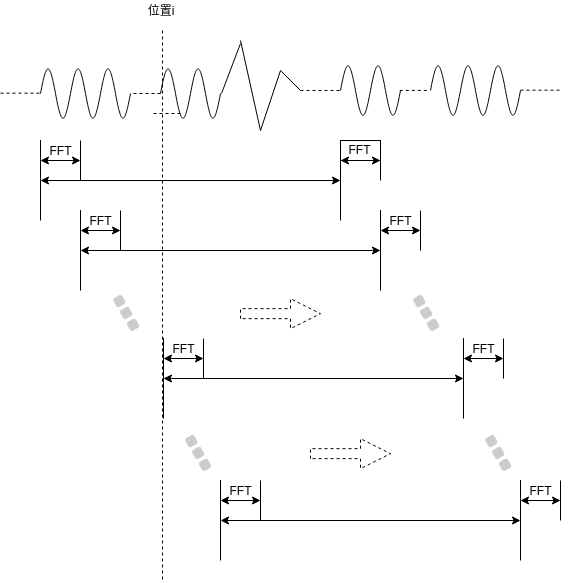
\includegraphics[width=0.6\textwidth]{images/detect_wave_algm}
    \caption{粗同步检波}{} % Crc Reconciliation
    \label{detect_wave_algm}
\end{figure}


\subsection{精同步}

在粗同步中,检波模块将检测到的导频信号转存到硬盘中,转存到硬盘的导频信号首尾两端是不完整的正弦波,首尾两端正弦波长度之和应该是$L_{sine_a}$,但是首部和尾部分别多长无法得知,因此需要进一步精确同步。

本文使用伪随机性序列(PN序列)作为精确同步和信道估计所用序列,由于m序列是PN序列中的一种,并且具有良好的自相关特性,所以本文使用m序列作为导频信号的主体部分。为了消除符号间干扰(Inter-Symbol-Interference,ISI)和载波间干扰(Inter-Carrier-Interference,ICI),在m序列后面添加循环前缀(Cyclic Prefix, CP)充当保护间隔,CP指的是将m序列的前面一部分复制到后段。

% TODO 加入仿真和实际测量中m序列自相关的图片
因为精同步发生在导频信号检测并转存之后,对实时性要求不高,因此本文利用m序列的自相关特性来精确切割导频信号。m序列的自相关函数是公式(\ref{m_self})所示周期性的二值函数,m序列的自相关函数时域上与冲激函数相近,在完全重合的周期点会出现波峰,并且随着m序列周期增加,m序列的随机性越好。设通信方转存的导频信号为$Rx$,包含的m序列理想情况为$m$,长度为$L_m$,第一段正弦波的完整长度为$L_{sine}$,那么可以遍历导频信号的起始一段,通过与已知原始m序列共轭相乘相加,求出波峰$Peak$并保存波峰位置i,

\begin{equation}
    Peak = max\{\frac{\sum_{k = i}^{L_m} \bar{m(k})\times Rx(i + k)}{L_m}) \}, i \in \{1, .., L_m + L_{sine}\}
\end{equation}

其中$\bar{\dot}$为取共轭。波峰$Peak$处对应的位置$i$就是精同步的结果,即m序列的起始位置,计算出m序列起始的精确位置,便可以进一步通过m序列或者其他数据段进行信道估计步骤。

图\ref{practical_pilot_m_seq}为系统转存的实际导频信号,其中包含第一段检波所用正弦波,以及m序列。通信方已知m序列原始信号如图\ref{m_seq}所示。图\ref{m_corr_practical}展示在实际系统中,转存信号中与已知m序列做相关的结果,其中根据波峰位置可以精确定位导频信号中m序列的起始位置。

\begin{figure}
    \centering
    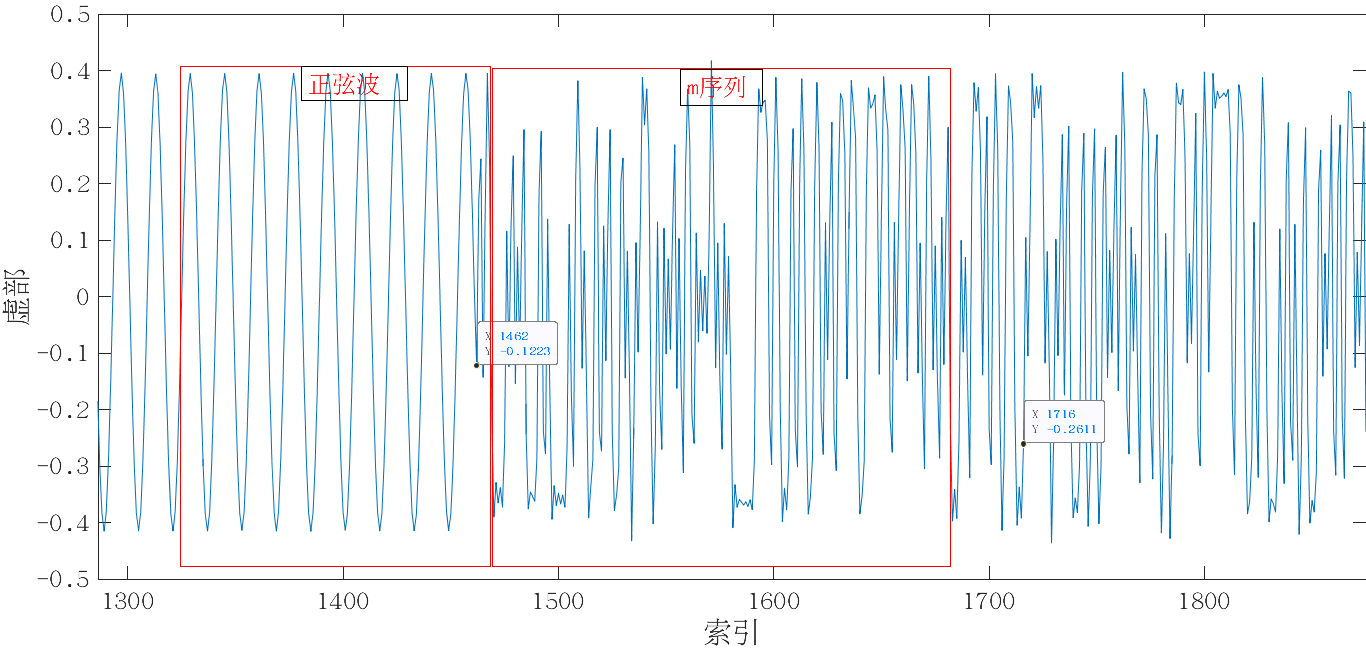
\includegraphics[width=0.9\textwidth]{images/practical_pilot_m_seq}
    \caption{实际导频信号中的m序列}{} 
    \label{practical_pilot_m_seq}
\end{figure}

\begin{figure}
    \centering
    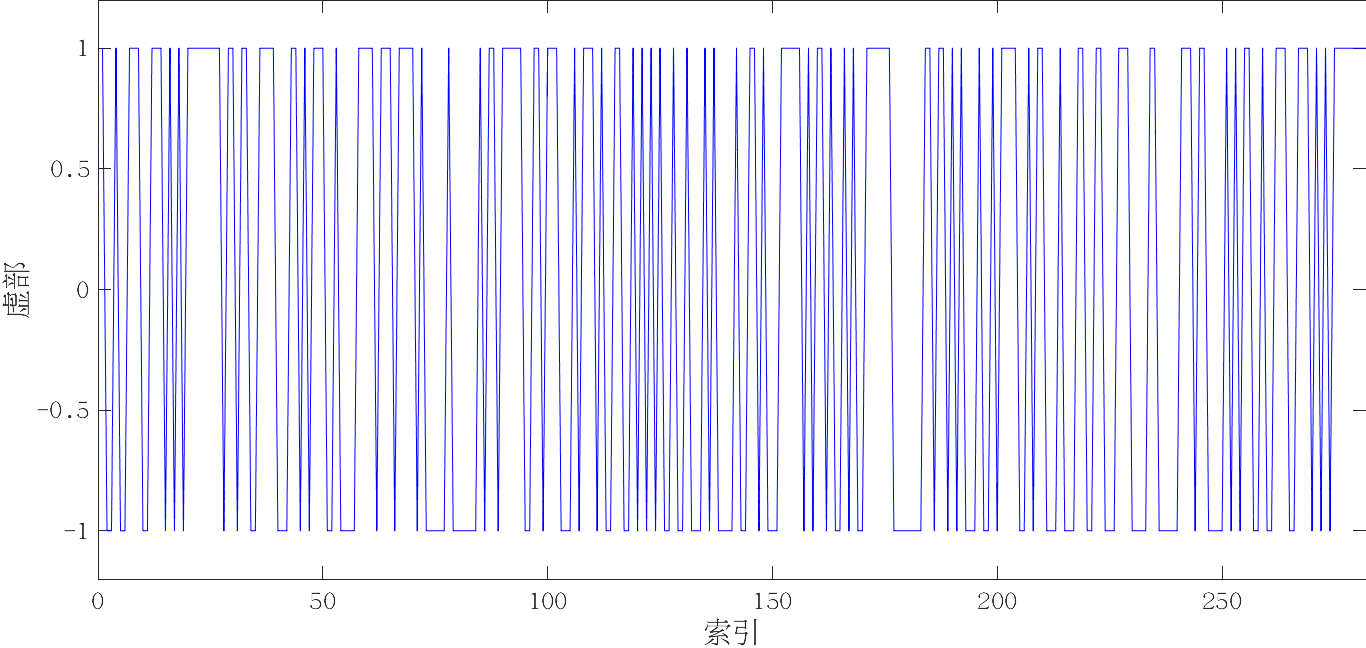
\includegraphics[width=0.9\textwidth]{images/m_seq}
    \caption{理想情况下的m序列}{} 
    \label{m_seq}
\end{figure}

\begin{figure}
    \centering
    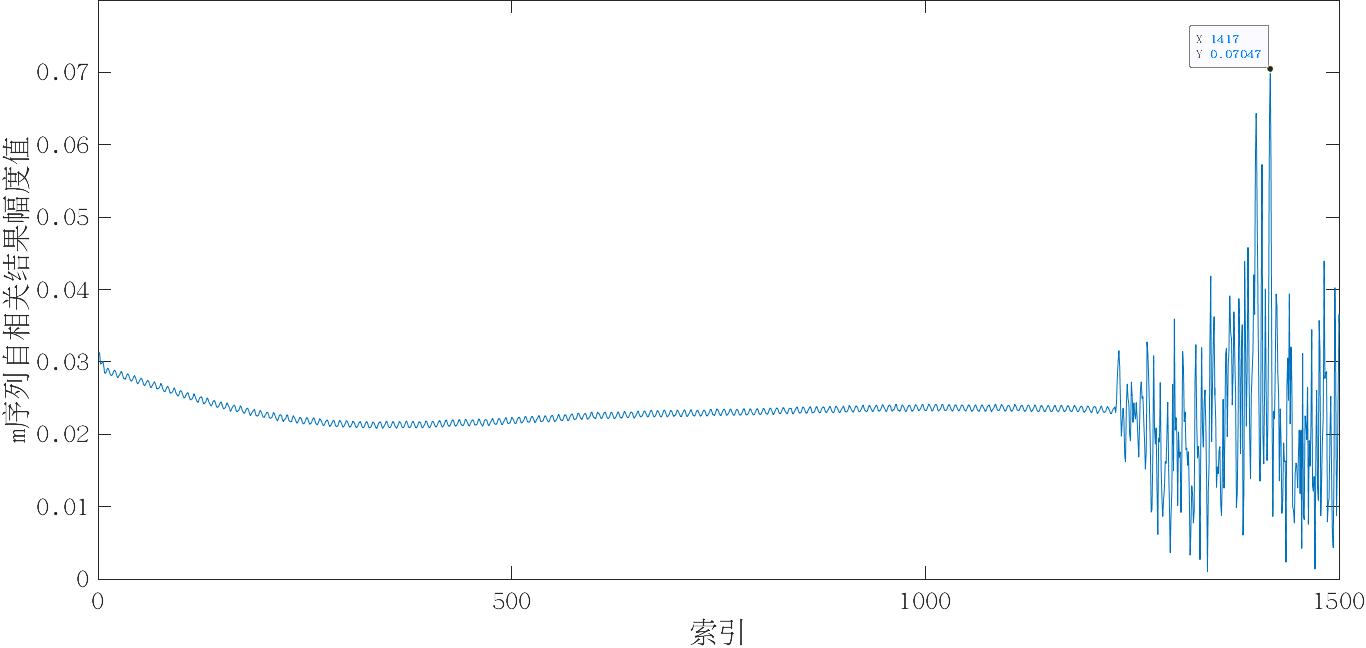
\includegraphics[width=0.9\textwidth]{images/m_corr_practical}
    \caption{理想和实际中m序列自相关}{} % Crc Reconciliation
    \label{m_corr_practical}
\end{figure}

\section{基于导频信号TDD收发系统设计}

本节阐述基于导频信号的TDD收发系统设计,从理论以及实现的角度详细介绍系统的构造。导频收发机是基于GNURadio搭建的,数据采集由USRP部分负责,USRP射频前端将数据转换到基带信号,并送入通用计算机中处理数据,实际上检波部分运行在计算机内,USRP将基带数据通过网口送入计算机内,计算机程序再去处理高速的数据流,并从中检测出导频信号。导频收发机是本系统最核心的部分,负责导频信号的发射、检测和转存。具体来说,由四个GNURadio模块构成:导频序列输出模块、数据发射模块、数据接收模块、导频信号检测模块。以下会详细介绍四个模块的实现。

\subsection{导频序列输出模块}

导频序列输出模块,可以理解为导频信号生成的模块,为方便起见,事先已经生成好导频信号存储在文件中,该模块可以直接读取该文件并送到输出端口。这种类型模块在GNURadio称作输出模块,输出模块无输出端口、有输出端口。本文为其设计了一个控制信号,即\ref{file_source_roi}图中所示$Tx\_File$这个布尔量,该模块内部有一状态量$Tx\_File\_$表示该模块是否正在发射数据。

\begin{itemize}
    \item 当$Tx\_File$设置为$True$时,该模块会检查$Tx\_File\_$变量查看当前是否输出数据。如果正在输出数据,则不做任何事情;如果不在输出数据,则会读取导频信号文件并送出到输出端口,当数据输出完成时,将$Tx\_File\_$设置为$False$
    \item 当$Tx\_File$设置为$False$时,该模块的输出端口不会输出任何数据。
\end{itemize}

因此,上层程序只需要控制$Tx\_File$这个变量,就可以控制导频信号的发射与否。将$Tx\_File$置为$True$,则会向输出端口送出导频信号(如果当前模块不在发射的话),置为$False$,则会立即停止输出任何数据。

\begin{figure}[htbp]
  \centering
  \subfloat[导频序列输出模块]{
      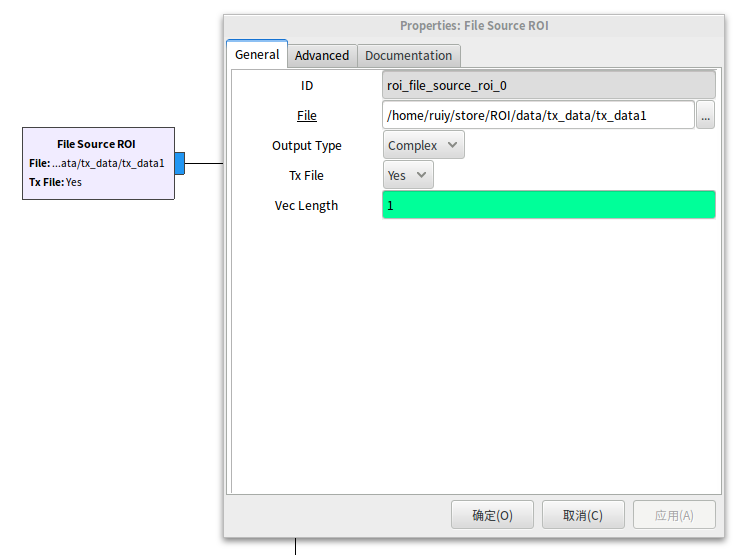
\includegraphics[width=0.48\textwidth]{images/file_source_roi}
      \label{file_source_roi}
  }
  \subfloat[数据发射模块]{
      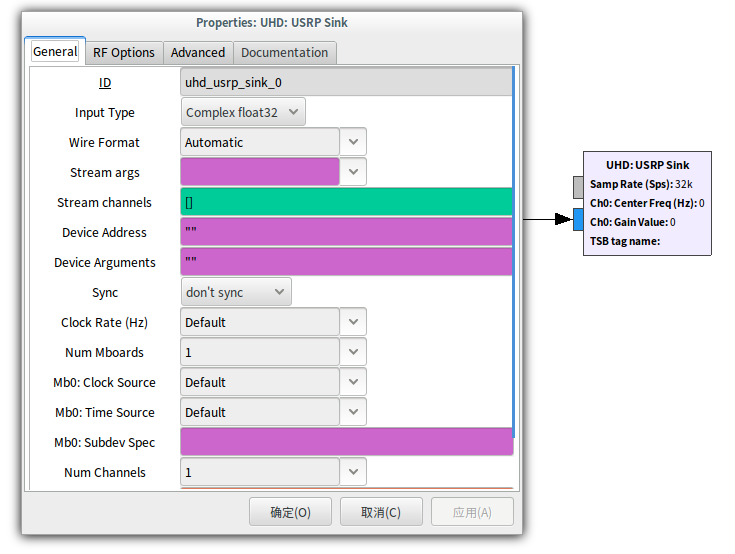
\includegraphics[width=0.48\textwidth]{images/usrp_sink}
      \label{usrp_sink}
  }
  \quad    %用 \quad 来换行
  \subfloat[数据接收模块]{
    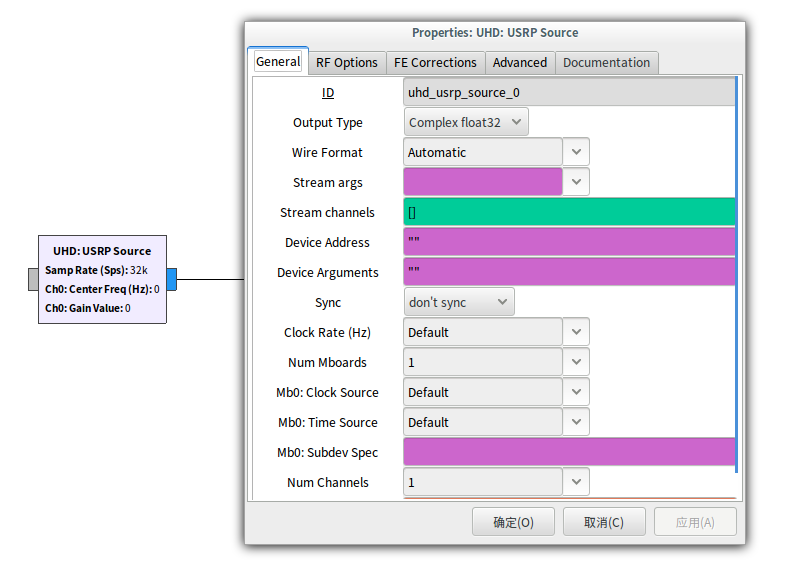
\includegraphics[width=0.48\textwidth]{images/usrp_source}
    \label{usrp_source}
  }
  \subfloat[导频信号检测模块]{
      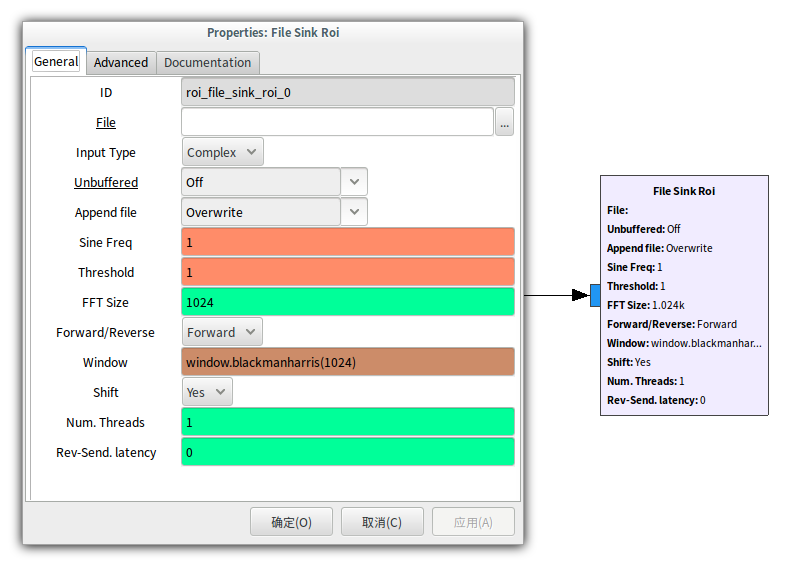
\includegraphics[width=0.48\textwidth]{images/file_sink_roi}
      \label{file_sink_roi}
  }
  \caption{导频信号收发机的四个模块}{} % xcorr between alice and bob, xcorr between bob and eve
  \label{four-block}
\end{figure}


\subsection{数据发射模块}

% 参考 https://zhuanlan.zhihu.com/p/24217098

数据发射模块是直接使用了GNURadio自带的模块$UHD: USRP\quad Sink$,其属于GNURadio的$gr-uhd$系列,该模块用于将数据采样点送入USRP设备中,USRP设备会将其调制发射到指定频率。其参数如图\ref{usrp_sink}所示。

该模块实际是计算机端的控制平台,其实际执行是由USRP中的FPGA以及相关器件实现实现。该模块需要将基带数据通过USB口或者网口送入到USRP中去,如图\ref{usrp_sink_theory}所示为PC端与USRP端的交互。该模块属于计算机端的上层应用程序,使用C++或者Python编写,调用UHD驱动程序和系统调用,控制硬件接口的数据读写。PC与USRP的交互使用USB3.0或者以太网网口,目前大部分外设均使用USB3.0或者千兆以太网网口传输数据,来保证输出速率,满足实时性,USB3.0的速率可达到500MBps\cite{wei2016software}。

在发射数据时,进程从用户态切换到内核态,通过系统调用控制网卡或USB的读写。通过以太网网口或者USB口,将数据送入到USRP内部。USRP内部的处理分为三个部分。

\begin{itemize}
    \item 首先,发送控制模块和数字上变频模块(DUC)为了处理速度足够快,采用FPGA实现。发送控制模块控制USRP的发送时序。DUC模块用于基带数据上变频到中频\cite{xiong2015open}。
    \item 其次,中频数字信号经过DAC器件数模转换得到模拟域的数据,再进一步进行模拟域的信号处理
    \item 模拟域中,信号先经过低通滤波器得到更加平滑的信号,再与晶振信号相乘,将中频信号调制到指定射频频点,最后射频信号经过功率放大器发射出去。
\end{itemize}


\subsection{数据接收模块}

数据接收模块也是直接使用了GNURadio内置的模块,同属于$gr-uhd$的模块集,该模块和$UHD: USRP\quad Sink$作用相反,其作用是通过USB口或者千兆以太网网口从USRP中获取基带数据,并送入到输出端口。其参数如图\ref{usrp_source}所示。


和$UHD: USRP\quad Sink$类似,该模块属于进程中的用户态部分,其在运行时会切换到内核态,并从与USRP相连接的以太网网口或者USB口读取高速数据。如图\ref{usrp_source_theory}所示为USRP在接收数据时与PC的交互。在接收数据时,USRP外设同样分为三个阶段处理信号,

\begin{itemize}
    \item 首先,信号经过低噪声放大器,避免将噪声放的过大。之后与晶振信号相乘,下变频到中频,再通过低通滤波器使得信号更加平滑。
    \item 其次,中频模拟信号通过ADC器件模数转换为数字信号。再进一步进行数字域的处理。
    \item 中频数字信号通过数字下变频,得到基带信号,再通过接收控制模块。为了速率保障,数字下变频模块和接收控制模块同样使用FPGA实现,接收控制模块控制USRP的接收行为。
\end{itemize}

USRP处理得到数字基带信号之后,通过以太网网口或者USB口,将数据送入PC中并触发中断,或者通知上层程序数据可读。PC中的上层程序陷入内核态,调用UHD驱动程序和系统调用从以太网网口或者USB口读取数据,然后返回用户态进一步处理数据。

\begin{figure}[htbp]
  \centering
  \begin{minipage}[t]{0.48\textwidth}
  \centering
  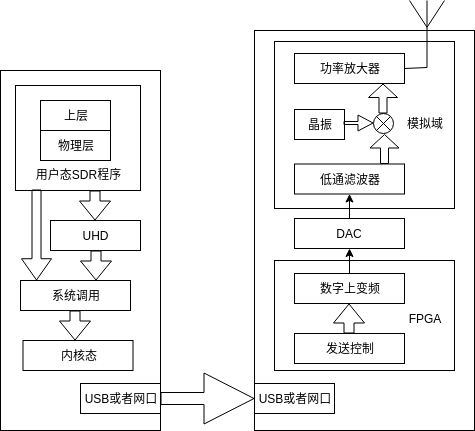
\includegraphics[width=6cm]{images/usrp_sink_theory}
  \caption{数据发射时USRP内部示意图}
  \label{usrp_sink_theory}
  \end{minipage}
  \begin{minipage}[t]{0.48\textwidth}
  \centering
  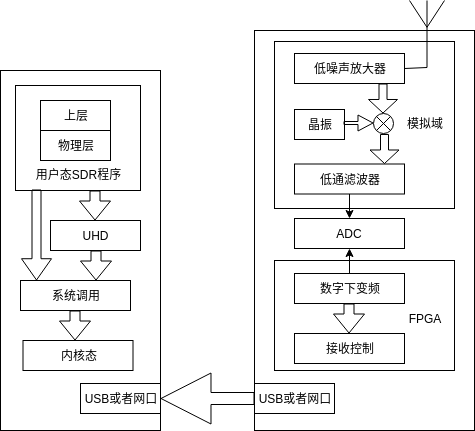
\includegraphics[width=6cm]{images/usrp_source_theory}
  \caption{数据接收时USRP内部示意图}
  \label{usrp_source_theory}
  \end{minipage}
\end{figure}

\subsection{导频信号检测模块}

导频信号检测模块从数据接收模块中读取基带数据流,并按照上述粗同步的方式,通过FFT检测指定间隔的两段信号是否为指定频率的正弦波,若是,则判断为需要检测的导频信号,将其转存到磁盘上,供之后信道估计使用。这种类型模块在GNURadio称作输入模块,输入模块无输出端口、有输入端口。

本文在设计该模块时提供了诸多模块参数,如图\ref{file_sink_roi}所示。其中各参数的意义为,

\begin{itemize}
    \item $Sine Freq$为该模块需要检测的导频信号首尾两端正弦波的频率
    \item $Threshold$为通过FFT判断能量时所用阈值
    \item $FFT Size$为检波是所做FFT长度
    \item $Rev-Send latency$为检测到导频信号与回发导频信号之间的时间间隔
\end{itemize}

通信双方的收发机中都有该模块。不同的是,当该模块检测到对端发射的导频信号,Bob会触发信号事件,将导频序列输出模块中的$Tx\_File$设置为$True$,发射Bob端的导频信号。Alice的导频信号检测模块收到Bob发射的导频信号之后,并不会再次发射信号,而是继续本次信道探测的后续过程,直到该次密钥生成过程完成,上层程序才会控制导频序列输出模块再次发射信号。


\subsection{导频信号收发机的整体结构}

本文基于上述四个GNURadio模块搭建导频信号收发机。上层程序通过控制Alice的导频序列发射模块,发射导频信号,将导频信号调制到指定频点,并通过USRP射频前端发射导频信号。Bob使用导频信号检测模块不断检测导频信号,当检测到指定导频信号时,转存到磁盘,并触发导频信号发射事件,通知发射机中的导频序列发射模块发射导频信号,Bob端的发射机发射导频信号之后,Alice端接收机中的导频信号检测模块可以检测到Bob端发射的导频信号,并转存导频信号到磁盘。一次信道探测过程完成。

实际上,检测算法由于阈值设定过高或者过低,有可能检测不到对方发射的导频信号或者将错误的信号数据误认为导频信号。因此Alice端设计了重发机制。在一次信道探测过程中,Alice会每隔一定时间,重新发射一次导频信号,直到检测到Bob回发的导频信号。

% \begin{figure}
%     \centering
%     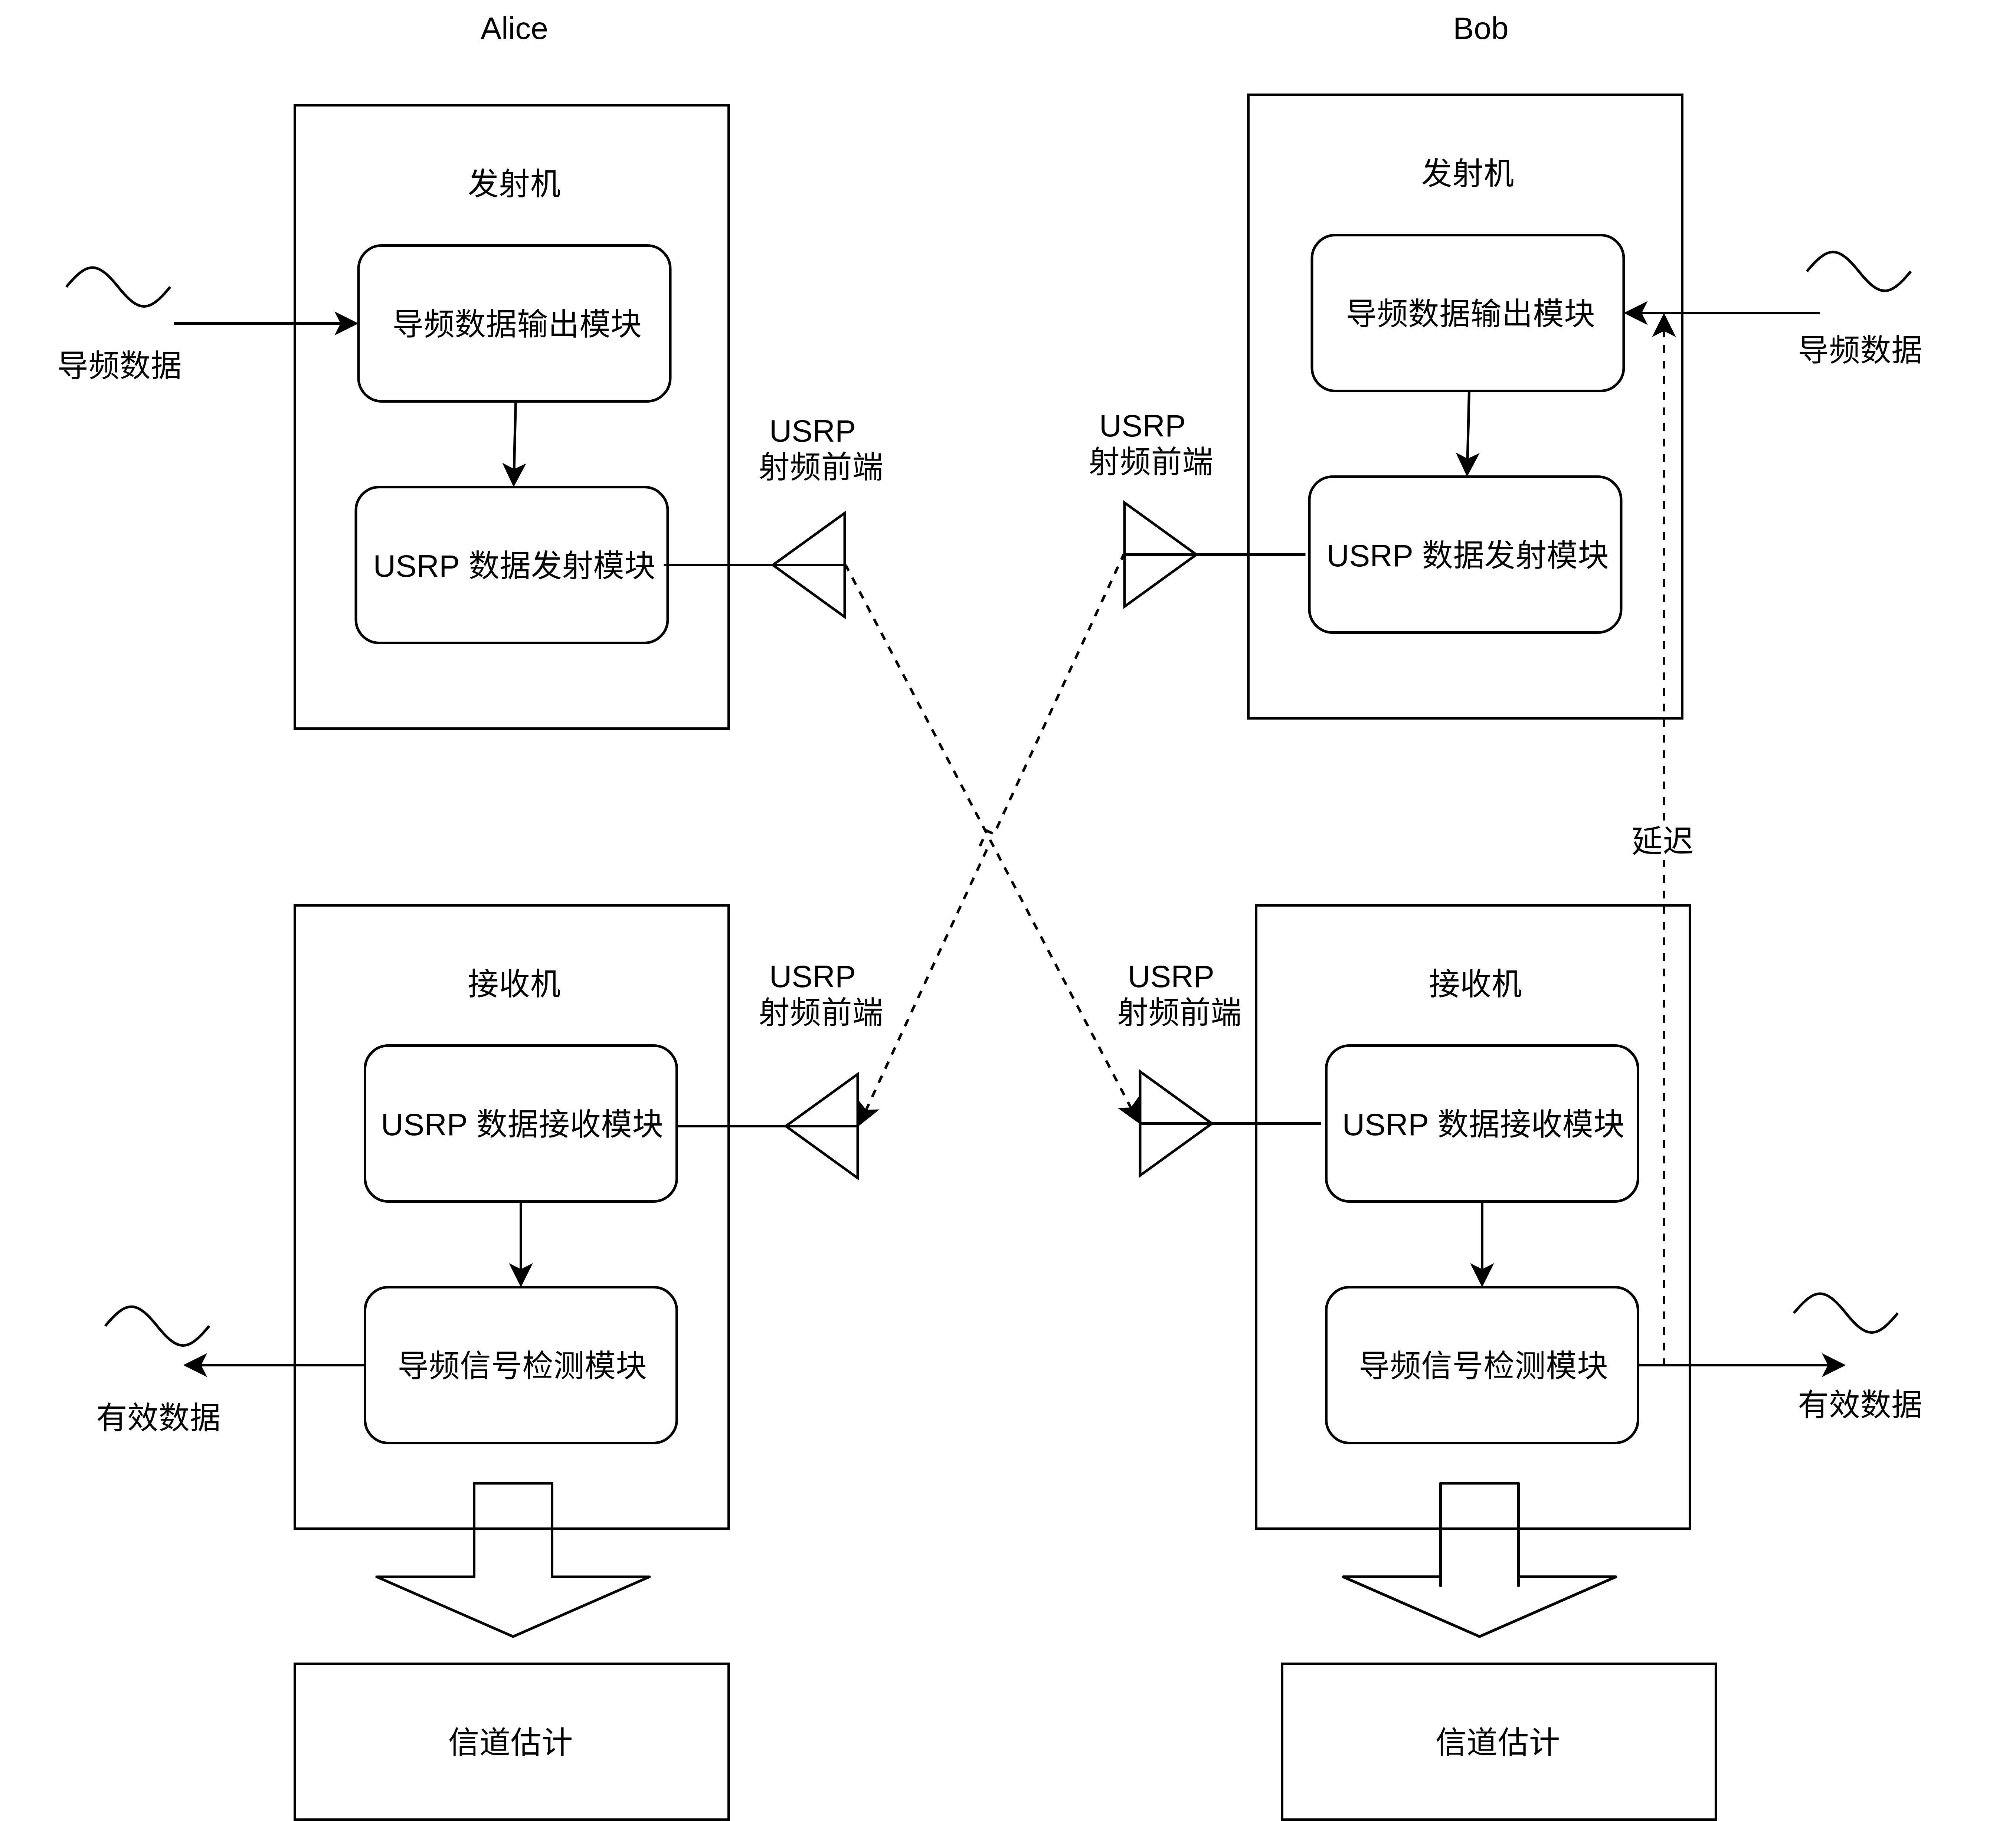
\includegraphics[width=0.9\textwidth]{images/two_tranceiver_structure2}
%     \caption{TDD导频收发机设计}{} 
%     \label{two_tranceiver_structure2}
% \end{figure}